\documentclass[aspectratio=169]{beamer}

\usetheme{Madrid}
\usecolortheme{default}

\usepackage{amsmath, amssymb}
\usepackage{booktabs}
\usepackage{tikz}
\usetikzlibrary{arrows.meta, positioning, fit, backgrounds}
\usepackage{listings}
\usepackage{xcolor}

\definecolor{codegray}{gray}{0.95}
\definecolor{codeblue}{RGB}{30,80,140}

\lstdefinestyle{Rstyle}{
  language=R,
  basicstyle=\ttfamily\small,
  backgroundcolor=\color{codegray},
  keywordstyle=\color{codeblue}\bfseries,
  commentstyle=\color{gray},
  stringstyle=\color{teal},
  showstringspaces=false,
  breaklines=true,
  frame=single,
  framerule=0pt,
  columns=fullflexible
}

\title[Topic Modeling]{Topic Modeling for Text Data}
\subtitle{From LDA to Structural Topic Models}
\author[McGee]{Monnie McGee}
\institute{REU Bootcamp}
\date{June 9, 2026}

\begin{document}

%------------------------------------------------
\begin{frame}
  \titlepage
\end{frame}

%------------------------------------------------
\begin{frame}{Today's Question}
\Large
Suppose we have thousands of documents.

\vspace{0.4cm}
How can we discover what people are talking about without reading every document?

\vspace{0.6cm}
\normalsize
Examples:
\begin{itemize}
  \item open-ended survey responses
  \item political speeches
  \item research abstracts
  \item news articles
  \item social media posts
\end{itemize}
\end{frame}

%------------------------------------------------
\begin{frame}{Learning Goals}
By the end of the session, you should be able to:

\begin{enumerate}
  \item Explain what a topic model is trying to estimate.
  \item Construct a document-term matrix.
  \item Interpret the LDA plate diagram.
  \item Fit and interpret a basic LDA model in R.
  \item Explain why Structural Topic Models extend LDA.
  \item Use document metadata to ask regression-style questions about topics.
\end{enumerate}
\end{frame}

%------------------------------------------------
\begin{frame}{Two-Hour Plan}
\begin{center}
\begin{tabular}{lll}
\toprule
Time & Segment & Mode \\
\midrule
0--15 & Text as data + warm-up exercise & discussion \\
15--30 & Latent variables and topics & presentation \\
30--50 & LDA plate diagram and generative story & presentation \\
50--65 & Preprocessing and DTM & R exercise \\
65--80 & Fit LDA in R & demonstration \\
80--95 & Interpreting topics & discussion \\
95--105 & Why LDA is incomplete & presentation \\
105--120 & Structural Topic Models & demo + exercise \\
\bottomrule
\end{tabular}
\end{center}
\end{frame}

%================================================
\section{Text as Data}

%------------------------------------------------
\begin{frame}{Documents, Words, and Topics}
\begin{block}{Basic idea}
A topic model treats each document as a mixture of latent themes called \textbf{topics}.
\end{block}

\vspace{0.3cm}
\begin{columns}
\column{0.48\textwidth}
\textbf{Document}
\begin{quote}
The economy added jobs, but inflation remains a concern.
\end{quote}

\column{0.48\textwidth}
\textbf{Possible topic mixture}
\begin{itemize}
  \item Economy: 70\%
  \item Labor: 20\%
  \item Politics: 10\%
\end{itemize}
\end{columns}
\end{frame}

%------------------------------------------------
\begin{frame}{Warm-Up Exercise: Discovering Topics by Hand}
\textbf{Instructions:} Working in pairs, read the eight mini-abstracts and identify the major themes.

\vspace{0.5em}
\small
\begin{enumerate}
  \item We investigate voting patterns in congressional elections using demographic and economic indicators.
  \item We develop a Bayesian model for predicting hospital readmission rates.
  \item We study climate change impacts on agricultural productivity across the Midwest.
  \item We propose a deep learning approach for medical image segmentation.
  \item We examine the relationship between air pollution and respiratory health.
  \item We analyze public attitudes toward environmental policy using survey data.
  \item We develop statistical methods for high-dimensional genomic data.
  \item We investigate machine learning techniques for climate forecasting.
\end{enumerate}
\end{frame}

%------------------------------------------------
\begin{frame}{Discussion: What Just Happened?}
Before we talk about topic models, consider the questions you just answered:

\begin{enumerate}
  \item How many topics are present?
  \item Does every document belong to exactly one topic?
  \item Which documents seem to belong to multiple topics?
  \item Could reasonable people disagree about the topics?
\end{enumerate}

\vspace{0.7em}
\pause

\begin{block}{Key idea}
Humans infer hidden topics from words. Topic models treat those topics as \emph{latent variables} and estimate them probabilistically.
\end{block}
\end{frame}

%------------------------------------------------
\begin{frame}{What Is a Latent Variable?}
A latent variable is a quantity that is not directly observed but is inferred from observed data.

\vspace{1em}
Examples:
\begin{itemize}
  \item intelligence inferred from test scores
  \item disease status inferred from symptoms
  \item customer satisfaction inferred from survey responses
  \item topic inferred from word usage
\end{itemize}

\vspace{1em}
\pause

In topic modeling:
\[
\text{Words observed}
\qquad \Longrightarrow \qquad
\text{Topics latent}
\]
\end{frame}

%================================================
\section{LDA}

%------------------------------------------------
\begin{frame}{Latent Dirichlet Allocation}
\Large
LDA says:

\vspace{0.4cm}
\begin{center}
\textbf{Documents are mixtures of topics.}\par
\textbf{Topics are mixtures of words.}
\end{center}

\vspace{0.5cm}
\normalsize
The model tries to infer both mixtures from the observed words.
\end{frame}

%------------------------------------------------
\begin{frame}{LDA Notation}
\begin{center}
\begin{tabular}{lll}
\toprule
Symbol & Meaning & Observed? \\
\midrule
$w_{dn}$ & word $n$ in document $d$ & yes \\
$z_{dn}$ & topic assignment for word $n$ in document $d$ & no \\
$\theta_d$ & topic mixture for document $d$ & no \\
$\beta_k$ & word distribution for topic $k$ & no \\
$\alpha$ & prior parameter for document-topic mixtures & fixed / estimated \\
$\eta$ & prior parameter for topic-word distributions & fixed / estimated \\
\bottomrule
\end{tabular}
\end{center}
\end{frame}



%------------------------------------------------
\begin{frame}{LDA Plate Diagram}

\begin{columns}[T]

\column{0.45\textwidth}

\centering

\begin{tikzpicture}[
node distance=0.9cm,
>=stealth,
every node/.style={font=\small}
]

\node (alpha) {$\alpha$};
\node (theta) [below=of alpha] {$\theta_d$};

\node (z) [below=of theta] {$z_{dn}$};
\node (w) [below=of z] {$w_{dn}$};

\node (eta) [right=2cm of alpha] {$\eta$};
\node (beta) [below=of eta] {$\beta_k$};

\draw[->] (alpha) -- (theta);
\draw[->] (theta) -- (z);
\draw[->] (z) -- (w);

\draw[->] (eta) -- (beta);
\draw[->] (beta) -- (w);

\end{tikzpicture}

\column{0.55\textwidth}

\small

\textbf{Observed}

\begin{itemize}
\item $w_{dn}$: observed word
\end{itemize}

\textbf{Latent}

\begin{itemize}
\item $\theta_d$: topic mixture
\item $z_{dn}$: topic assignment
\item $\beta_k$: topic-word distribution
\end{itemize}

\textbf{Read arrows as:}

\begin{itemize}
\item $\theta_d \rightarrow z_{dn}$
\item $\beta_k \rightarrow w_{dn}$
\item $z_{dn} \rightarrow w_{dn}$
\end{itemize}

\end{columns}

\end{frame}

%------------------------------------------------
\begin{frame}{LDA Plate Diagram: Formal Version}

\centering

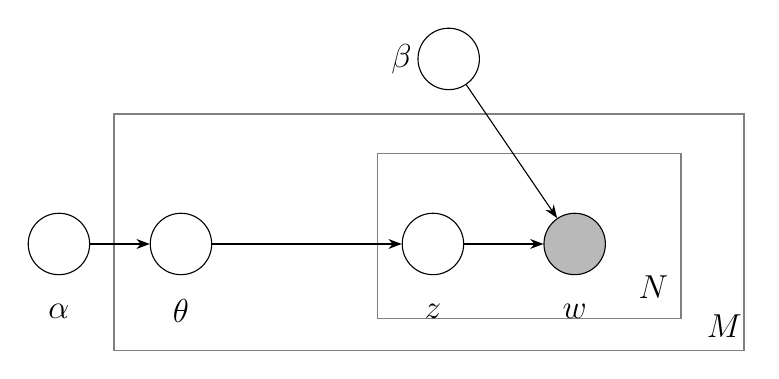
\begin{tikzpicture}[
    >=Stealth,
    node/.style={circle, draw, minimum size=0.78cm, inner sep=0pt},
    obs/.style={circle, draw, fill=gray!55, minimum size=0.78cm, inner sep=0pt},
    every node/.style={font=\large}
]

% Plates
\draw[gray] (-2.3,-1.35) rectangle (5.7,1.65);
\draw[gray] (1.05,-0.95) rectangle (4.9,1.15);

% Nodes
\node[node] (alpha) at (-3.0,0) {};
\node[node] (theta) at (-1.45,0) {};
\node[node] (z)     at (1.75,0) {};
\node[obs]  (w)     at (3.55,0) {};
\node[node] (beta)  at (1.95,2.35) {};

% Arrows
\draw[->] (alpha) -- (theta);
\draw[->] (theta) -- (z);
\draw[->] (z) -- (w);
\draw[->] (beta) -- (w);

% Labels
\node[draw=none] at (-3.0,-0.85) {$\alpha$};
\node[draw=none] at (-1.45,-0.85) {$\theta$};
\node[draw=none] at (1.75,-0.85) {$z$};
\node[draw=none] at (3.55,-0.85) {$w$};
\node[draw=none] at (1.35,2.35) {$\beta$};

% Plate labels
\node[draw=none] at (4.55,-0.55) {$N$};
\node[draw=none] at (5.45,-1.05) {$M$};

\end{tikzpicture}

\vspace{0.75em}

\footnotesize
\textbf{Source:} Blei, D. M., Ng, A. Y., \& Jordan, M. I. (2003).
\emph{Latent Dirichlet Allocation}. 
\emph{Journal of Machine Learning Research}, 3, 993--1022.

\end{frame}
%------------------------------------------------
\begin{frame}{What Are We Trying to Estimate?}
We observe only the words in each document.

\vspace{0.4cm}
\begin{center}
\begin{tabular}{lll}
\toprule
Quantity & Interpretation & Why we care \\
\midrule
$\theta_d$ & topic mixture for document $d$ & summarizes documents \\
$\beta_k$ & word distribution for topic $k$ & helps label topics \\
$z_{dn}$ & topic assignment for word $n$ & links words to topics \\
\bottomrule
\end{tabular}
\end{center}

\vspace{0.5cm}
\begin{block}{Inference problem}
Given only the observed words $w_{dn}$, can we estimate the hidden quantities?
\end{block}
\end{frame}

%------------------------------------------------
\begin{frame}{The Generative Story}
For each topic:
\[
\beta_k \sim \text{Dirichlet}(\eta)
\]

For each document:
\[
\theta_d \sim \text{Dirichlet}(\alpha)
\]

For each word position:
\[
z_{dn} \sim \text{Categorical}(\theta_d)
\]
\[
w_{dn} \sim \text{Categorical}(\beta_{z_{dn}})
\]
\end{frame}

%------------------------------------------------
\begin{frame}{Connecting the Diagram to the Probability Model}
\[
P(w,z,\theta,\beta)
=
\prod_k P(\beta_k)
\prod_d P(\theta_d)
\prod_n
P(z_{dn}\mid \theta_d)
P(w_{dn}\mid z_{dn},\beta)
\]

\vspace{0.4cm}
\begin{block}{Takeaway}
Each arrow in the plate diagram corresponds to a conditional distribution in the joint model.
\end{block}
\end{frame}

%------------------------------------------------
\begin{frame}{Two Kinds of Probabilities}
\begin{columns}
\column{0.48\textwidth}
\textbf{Document-topic probabilities}

\begin{center}
\begin{tabular}{lr}
\toprule
Topic & Probability \\
\midrule
Economy & 0.60 \\
Health & 0.25 \\
Foreign policy & 0.15 \\
\bottomrule
\end{tabular}
\end{center}

\column{0.48\textwidth}
\textbf{Topic-word probabilities}

\begin{center}
\begin{tabular}{lr}
\toprule
Word & Probability \\
\midrule
jobs & 0.08 \\
inflation & 0.07 \\
wages & 0.05 \\
market & 0.04 \\
\bottomrule
\end{tabular}
\end{center}
\end{columns}
\end{frame}

%================================================
\section{Preprocessing}

%------------------------------------------------
\begin{frame}{From Text to Data}
To fit the model, we need to transform raw text into a form the computer can use.

\vspace{0.2cm}
Common steps:
\begin{itemize}
  \item tokenize documents into words
  \item remove stop words
  \item remove punctuation, numbers, or rare words
  \item optionally stem or lemmatize words
  \item create a document-term matrix
\end{itemize}

\vspace{0.3cm}
\begin{block}{Important warning}
Preprocessing choices are modeling choices. They can change the topics you discover.
\end{block}
\end{frame}

%------------------------------------------------
\begin{frame}{Document-Term Matrix}
\begin{center}
\begin{tabular}{lrrrrr}
\toprule
Document & economy & jobs & health & vote & climate \\
\midrule
Doc 1 & 2 & 1 & 0 & 0 & 0 \\
Doc 2 & 0 & 0 & 3 & 0 & 0 \\
Doc 3 & 1 & 0 & 0 & 2 & 1 \\
Doc 4 & 0 & 0 & 0 & 1 & 4 \\
\bottomrule
\end{tabular}
\end{center}

\vspace{0.4cm}
Rows are documents. Columns are words. Entries are word counts.
\end{frame}


%------------------------------------------------
\begin{frame}[fragile]{R Exercise: Tokenize Text}
\begin{lstlisting}[style=Rstyle]
library(tidyverse)
library(tidytext)

documents <- read_csv("abstracts.csv")

tokens <- documents %>%
  unnest_tokens(word, text) %>%
  anti_join(stop_words, by = "word")

tokens %>%
  count(word, sort = TRUE)
  \end{lstlisting}

\vspace{0.2cm}
Exercise:
\begin{itemize}
  \item What are the most common words?
  \item Are there words you would add to a custom stop-word list?
\end{itemize}
\end{frame}

%------------------------------------------------
\begin{frame}[fragile]{Preprocessing: From Text to a Document-Term Matrix}

\small
\begin{lstlisting}[style=Rstyle]
documents <- read_csv("abstracts.csv")

tokens <- documents %>%
  unnest_tokens(word, text) %>%
  anti_join(stop_words, by = "word")

word_counts <- tokens %>%
  count(id, word)

dtm <- word_counts %>%
  cast_dtm(document = id,
           term = word,
           value = n)
\end{lstlisting}

\vspace{0.2cm}

\centering
Raw Text $\rightarrow$ Tokenization $\rightarrow$ Remove Stop Words  $\rightarrow$ Word Counts $\rightarrow$ DTM
\end{frame}
%------------------------------------------------
\begin{frame}[fragile]{Fitting an LDA Topic Model}

\small

\textbf{Goal:} Discover latent topics from the document-term matrix.

\vspace{0.3cm}

\begin{columns}[T]

\column{0.62\textwidth}

\begin{lstlisting}[style=Rstyle]
library(topicmodels)

# Fit a topic model with 5 topics
lda_fit <- LDA(
  dtm,
  k = 5,
  control = list(seed = 1234)
)

# Display the 10 most probable
# words for each topic
terms(lda_fit, 10)
\end{lstlisting}

\column{0.38\textwidth}

\pause

%\begin{block}{Discussion Questions}
%\begin{itemize}
  %  \item Why did we choose $k = 5$?
   % \item What if $k = 3$?
   % \item What if $k = 10$?
    %\item Do the topics make sense?
%\end{itemize}
%\end{block}

\begin{tikzpicture}[remember picture,overlay]

\node[
    fill=yellow!15,
    draw,
    rounded corners,
    text width=4cm,
    align=left
]
at (1,-2)
{
\textbf{Discussion}

\begin{itemize}
\item Why $k=5$?
\item What if $k=3$?
\item What if $k=10$?
\end{itemize}
};

\end{tikzpicture}
\end{columns}

\end{frame}

%------------------------------------------------
\begin{frame}[fragile]{Visualize Top Words by Topic}
\begin{lstlisting}[style=Rstyle]
beta <- tidy(lda_fit, matrix = "beta")

beta %>%
  group_by(topic) %>%
  slice_max(beta, n = 10) %>%
  ungroup() %>%
  ggplot(aes(beta, reorder_within(term, beta, topic))) +
  geom_col() +
  facet_wrap(~ topic, scales = "free") +
  scale_y_reordered()
\end{lstlisting}
\end{frame}

%================================================
\section{Why LDA Is Incomplete}

%------------------------------------------------
\begin{frame}{What LDA Ignores}

Suppose we know something about each document.

\vspace{0.4cm}

Examples:

\begin{itemize}
  \item year written
  \item political party
  \item country
  \item author gender
  \item treatment group
  \item publication source
\end{itemize}

\vspace{0.4cm}

Where does that information enter the LDA model?

\pause

\pause

\begin{tikzpicture}[remember picture,overlay]

\node[
    fill=yellow!20,
    draw,
    rounded corners,
    text width=5cm,
    align=center
]
at (8,3)
{
\Huge\bfseries Nowhere.
\vspace{0.5cm}

\Large
LDA only sees words.
};

\end{tikzpicture}

\end{frame}
%------------------------------------------------
\begin{frame}{The Statistical Problem}
LDA can tell us what topics appear in documents.

\vspace{0.3cm}
But researchers often want to ask:

\begin{itemize}
  \item Are some topics more common among one group than another?
  \item Do topics become more or less prevalent over time?
  \item Does an experimental treatment affect what people write about?
  \item Do different groups use different words when discussing the same topic?
\end{itemize}

\vspace{0.4cm}
These are regression-style questions.
\end{frame}

%================================================
\section{Structural Topic Models}

%------------------------------------------------
\begin{frame}{Structural Topic Models}
\begin{block}{STM extends LDA}
Structural Topic Models allow document-level metadata to influence topic prevalence and, optionally, topic content.
\end{block}

\vspace{0.3cm}
Two major uses of metadata:
\begin{itemize}
  \item \textbf{Topic prevalence}: which topics are more common?
  \item \textbf{Topic content}: what words are used within a topic?
\end{itemize}
\end{frame}

%------------------------------------------------
\begin{frame}{STM as a Regression Extension}
In LDA:
\[
\theta_d \sim \text{Dirichlet}(\alpha)
\]

In STM, conceptually:
\[
\theta_d = f(X_d)
\]

where $X_d$ contains document-level covariates.

\vspace{0.4cm}
Examples:
\[
X_d = \{\text{party}, \text{year}, \text{treatment group}\}
\]
\end{frame}

%------------------------------------------------
\begin{frame}{Conceptual STM Diagram}

\begin{columns}[T]

\column{0.55\textwidth}

\centering
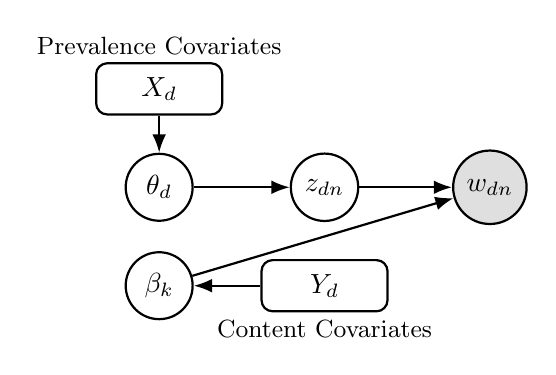
\begin{tikzpicture}[
    latent/.style={circle, draw, thick, minimum size=0.85cm},
    observed/.style={circle, draw, thick, fill=gray!25, minimum size=0.85cm},
    box/.style={rectangle, draw, thick, rounded corners,
                minimum width=1.6cm, minimum height=0.65cm},
    arrow/.style={-Latex, thick}
]

% Main chain
\node[latent] (theta) at (0,0) {$\theta_d$};
\node[latent] (z) at (2.1,0) {$z_{dn}$};
\node[observed] (w) at (4.2,0) {$w_{dn}$};

\draw[arrow] (theta) -- (z);
\draw[arrow] (z) -- (w);

% Prevalence covariates
\node[box] (X) at (0,1.25) {$X_d$};
\draw[arrow] (X) -- (theta);

\node[align=center,font=\small]
at (0,1.8)
{Prevalence Covariates};

% Content covariates
\node[box] (Y) at (2.1,-1.25) {$Y_d$};
\node[latent] (beta) at (0,-1.25) {$\beta_k$};

\draw[arrow] (Y) -- (beta);
\draw[arrow] (beta) -- (w);

\node[align=center,font=\small]
at (2.1,-1.8)
{Content Covariates};

\end{tikzpicture}

\column{0.45\textwidth}

\vspace{0.7cm}

\begin{block}{Interpretation}
\small
\begin{itemize}
\item $X_d$: affects which topics appear in a document.

\vspace{0.35cm}

\item $Y_d$: affects how topics are expressed through words.
\end{itemize}
\end{block}

\end{columns}

\end{frame}

%------------------------------------------------
\begin{frame}[fragile]{STM: Incorporating Document Metadata}

\small

\begin{columns}[T]

\column{0.5\textwidth}


\begin{lstlisting}[style=Rstyle]
library(readr)
library(stm)

abstracts <- read_csv("abstracts.csv")

# Add document metadata (I made this up)
abstracts$field <- c(
  "policy", "health",
  "environment", "health",
  "environment", "policy",
  "statistics",
  "environment"
)
\end{lstlisting}

\column{0.5\textwidth}
\begin{lstlisting}[style=Rstyle]
processed <- textProcessor(
  documents = abstracts$text,
  metadata  = abstracts
)

\end{lstlisting}
\end{columns}
\end{frame}

%------------------------------------------------

\begin{frame}[fragile]{STM: Fitting the Model}


\small

\begin{columns}[T]

\column{0.62\textwidth}

\begin{lstlisting}[style=Rstyle]
out <- prepDocuments(
  processed$documents,
  processed$vocab,
  processed$meta
)

stm_fit <- stm(
  documents = out$documents,
  vocab     = out$vocab,
  K   =  5,
  prevalence = ~ field,
  data      = out$meta,
  seed      = 1234
)
\end{lstlisting}

\column{0.38\textwidth}

\begin{block}{Key Difference from LDA}

LDA only uses:

\begin{itemize}
\item words
\end{itemize}

STM uses:

\begin{itemize}
\item words
\item document metadata
\end{itemize}

\end{block}

\vspace{0.2cm}

\pause

\begin{alertblock}{Important Line}

\centering
\texttt{prevalence = \textasciitilde{} field}

\end{alertblock}

This allows topic prevalence to depend on the document's field.

\end{columns}

\end{frame}
%------------------------------------------------
\begin{frame}[fragile]{Estimate Effects of Metadata}
\begin{lstlisting}[style=Rstyle]
effects <- estimateEffect(
  1:5 ~ field,
  stm_fit,
  meta = out$meta
)

summary(effects)
plot(effects, covariate = "field", topics = c(1, 3, 5))
\end{lstlisting}

\vspace{0.3cm}
Exercise:
\begin{itemize}
  \item Choose one topic.
  \item Estimate whether its prevalence differs by metadata group.
  \item Interpret the result in ordinary language.
\end{itemize}
\end{frame}

%------------------------------------------------
\begin{frame}{LDA vs. STM}
\begin{center}
\begin{tabular}{lll}
\toprule
Feature & LDA & STM \\
\midrule
Uses words & yes & yes \\
Latent topics & yes & yes \\
Document-topic mixtures & yes & yes \\
Metadata affects topic prevalence & no & yes \\
Metadata affects topic content & no & optional \\
Regression-style interpretation & limited & central \\
\bottomrule
\end{tabular}
\end{center}
\end{frame}

%-----------------------------------------------

\begin{frame}[fragile]{Choosing the Number of Topics ($K$)}

\small

\begin{columns}[T]

\column{0.48\textwidth}

\begin{block}{LDA}

Fit models for several values of $K$.

\begin{lstlisting}[style=Rstyle]
result <- FindTopicsNumber(
  dtm,
  topics = 2:10
)
FindTopicsNumber
plot( result)
\end{lstlisting}

Evaluate:

\begin{itemize}
\item Semantic coherence
\item Topic interpretability
\end{itemize}

\end{block}

\column{0.48\textwidth}

\begin{block}{STM}

Use built-in diagnostics.

\begin{lstlisting}[style=Rstyle]
k_result <- searchK(
  documents =
    out$documents,
  vocab =
    out$vocab,
  K = c(3,5,7,10)
)
plot(k_result)
\end{lstlisting}

Evaluate:

\begin{itemize}
\item Semantic coherence
\item Exclusivity
\end{itemize}

\end{block}

\end{columns}

\end{frame}

%------------------------------------------------
\begin{frame}{Choosing the Number of Topics}

\centering
Statistical criteria can help narrow the range of
reasonable values, but interpretability and scientific
usefulness still matter.

\pause
\vspace{0.3cm}
\renewcommand{\arraystretch}{1.4}

\begin{tabular}{|p{5cm}|p{7cm}|}
\hline
\textbf{Diagnostic} & \textbf{Question} \\
\hline
Semantic Coherence &
Do the top words tend to occur together in documents? \\
\hline
Exclusivity &
Do the top words distinguish this topic from the others? \\
\hline
\end{tabular}

\vspace{0.3cm}
\pause
\centering
\begin{alertblock}{Important}
There is rarely a single correct value of $K$. A useful topic model balances semantic coherence and exclusivity.
\end{alertblock}


\end{frame}
%------------------------------------------------
\begin{frame}{Interpretation Checklist}
For any topic model, ask:

\begin{enumerate}
  \item Are the top words coherent?
  \item Can we give the topic a meaningful name?
  \item Which documents are most associated with the topic?
  \item Is the topic stable across reasonable choices of $K$?
  \item Are metadata effects substantively meaningful?
  \item What preprocessing choices might have affected the result?
\end{enumerate}
\end{frame}

%------------------------------------------------
\begin{frame}{Mini-Project}
In small groups using either the folktales data or the nsf\_abstracts data:

\begin{enumerate}
  \item Fit an LDA or STM model.
  \item Choose a value of $K$ and justify it.
  \item Name 3--5 topics.
  \item Identify one interesting document for a topic.
  \item If using STM, interpret one metadata effect.
\end{enumerate}

\vspace{0.4cm}
Prepare a two-minute report:

\begin{quote}
What did the model reveal, and what should we be cautious about?
\end{quote}
\end{frame}

%------------------------------------------------
\begin{frame}{Closing Thought}

\Large

Topic models are not machines that discover truth.

\vspace{0.5cm}

They are statistical tools for organizing, summarizing, and questioning large collections of text.

\vspace{0.6cm}

\begin{alertblock}{Research Requires Judgment}
The analyst still has to choose the model, evaluate the results, and justify the conclusions.
\end{alertblock}

\end{frame}

\end{document}
